
\documentclass{TDP005mall}
\usepackage[utf8]{inputenc}
\usepackage[swedish]{babel}


\newcommand{\version}{Version 1.2}
\author{Daniel Huber, \url{danhu849@student.liu.se}\\
  Jens �hrnell, \url{jenoh242@student.liu.se}}
\title{Dokumentmall}
\date{2020-11-18}
\rhead{Daniel Huber\\
Jens �hrnell}



\begin{document}
\projectpage
\tableofcontents
\section{Revisionshistorik}
\begin{table}[!h]
\begin{tabularx}{\linewidth}{|l|X|l|}
\hline
Ver. & Revisionsbeskrivning & Datum \\\hline
1.2 & Kravspecifikation TDP005 & 201118 \\\hline
1.1 & Modifierad för att stödja xelatex och unicode & 150603 \\\hline
1.0 & Skapad för studenter att använda som mall till
kommande dokumentinlämningar & 140908 \\\hline
\end{tabularx}
\end{table}


\section{Spelide´}% Hur skriver man e med apostrof i latex..?
% Vad går spelet ut på? - Tänk: vad ska stå på Steam-sidan som säljer ert spel?
Din familj har kidnappads av Ondskan! Du vet om att Ondskan håller till på toppen av berg omgivna av lava, men du vet inte vilket! Klättra upp för bergen genom att hoppa upp på plattformarna, undvik den ökande nivån av lava, döda eller undvik fienderna, samla power-ups och besegra bossen på toppen av berget! I denna bottom-top platforms scroller kan du spela ensam eller tillsammans med en vän. Klara banorna snabbare för högre highscore. Kan du rädda din familj i tid?

Spelaren/spelarna börjar på botten av berget vid varje nivås början med fullt liv och en pistol. Efter att ha hoppat upp på första platformen börjar lavan stiga och spelarfönstret börjar förflytta sig uppåt. I takt med att spelarfönstret och spelaren rör sig uppåt så uppkommer fler platformar spelaren kan hoppa upp till. Fiender kan finnas och röra sig över platformarna samt skjuta i bestämda tidsintervall eller när spelaren befinner sig på samma höjd som dem. Fiender kan också flyga i utrymmet mellan plattformarna. Spelaren kan inte röra sig utanför skärmen och kan inte hoppa igenom plattformar. Får spelaren noll liv eller rör lavan så är det game over. På plattformarna kan också power-ups finnas som aktiveras när spelaren går i samma ruta som dem. Dessa kan ge antingen permanenta eller temporära fördelar i nivån, men förs inte över till nästa nivå.


\subsection{Spelets mål}
Spelarens mål är att överleva, klättra upp till toppen av berget och rädda familjen.

\section{Målgrupp}% Vilka typer av spelare borde spela ert spel?
Spelet riktas mot spelare som tycker om speluppgifter som måste klaras av under en viss tid.

\section{Spelupplevelse}% Vad gör spelet underhållande att spela?
Spelaren tvingas i varje nivå hitta den mest tidseffektiva vägen upp samtidigt som fiender och dess projektiler undviks. Vid avklarande belönas spelaren med en känsla utav att ha klarat av en utmaning.  

\section{Spelmekanik}% Hur interagerar man med spelet? Vilka kommandon? Vad driver spelet framåt?


\subsection{Förflyttning}

\begin{table}[!h]
  \caption{Tangentbordskommandon\label{tab}}
\begin{tabularx}{\linewidth}{|l|l|}
\hline
Tangent & Resultat \\\hline
↑, Z & Spelaren hoppar uppåt. \\\hline
← & Spelaren förflyttas åt vänster. \\\hline
→ & Spelaren förflyttas åt höger. \\\hline
↑ + ←, Z + ← & Spelaren hoppar åt vänster. \\\hline
↑ + →, Z + → & Spelaren hoppar åt höger. \\\hline
X & Ett skott avfyras i den riktningen spelaren är vänd åt. \\\hline
\end{tabularx}
\end{table}


% Lägg till gamepad ifall vi bestämmer oss för det - i bör-kraven.
Spelaren styrs med hjälp av tangentbordet enligt tabellen \ref{tab} nedan och kan förflyttas åt höger eller vänster både på marken och i luften. Spelare kan välja att hoppa åt både vänster, höger och rakt upp. Det finns bara en hopphöjd och denna är oföränderlig. Spelaren bygger vid rörelse åt något håll upp momentum så när spelaren släpper tangenten fortsätter spelarkaraktären förflytta sig en liten bit till.

\subsection{Fiender}
Fiender är antingen stationära eller rör sig i förutbestämda mönster. De kan finnas på platformar eller i luften mellan platformarna. Det finns tre typer av fiender. En flygande typ, en gående typ och en hoppande typ.

\subsection{Vapen}
Spelaren kan med tangentbordstryckning avfyra projektiler från sin medhavda pistol. Med denna ges spelaren möjlighet att försvara sig och döda fiender i varje nivå. 

\subsection{Spelarfönstret}
Spelarfönstret följer hela tiden spelaren så om spelaren rör sig snabbare uppåt än lavan kan lavan hamna ur bild. Den nedersta delen av spelarfönstret upptas av lava. Spelare och fiender som rör vid lavan dör genast. Stannar spelaren för länge på samma höjd tar lavan över ett allt större område på spelskärmen. 


\subsection{Spelmeny}
Det första spelaren möts av efter programmets start är spelets meny i form av knappar. Spelaren kan manövrera över knapparna med piltangenterna och välja med mellanslag. Spelaren kan välja mellan en nivåmeny, inställningar för att se tangentkommandon samt att stänga av spelets musik och ljud och ytterligare en knapp med information över skaparna av spelet.  \ref{REFERENS TILL VISUALISERING} 

\section{Regler}% Vilka regler styr spelet?

\subsection{Single player}
Spelaren har vid varje nivås början tre liv som finns representerade i en health-bar i övre delen av spelarfönstret. Vid fullt liv kan extra liv plockas upp, men de fyller inte på med mer liv än de tre som är max. Förloraren spelaren alla liv visas game over. Vid kontakt med fiendeprojektiler tar spelaren ett i skada.

\subsection{Multiplayer} % möjlig implementation.


\subsection{Fiender}
Fiendetyper som kan avfyra projektiler gör de så under regelbundna tidsintervall. Dör en fiende efter att ha avfyrat ett skott så fortsätter fiendens skott tills det träffar något eller åker utanför banan. Vid fiendens död försvinner fienden. Fiender skadar spelaren ett liv.

\subsection{Power-ups}
Power-ups finns förutbestämt utlagda på plattformarna sedan innan. De är en del av nivån.

\subsection{Projektiler}
Skott som avfyras med spelarens vapen kan bara skjutas åt det håll spelaren är vänd åt, antingen höger eller vänster. Spelaren kan inte skjuta uppåt. Skotten flyger rakt och förflyttas ej i y-led. Avfyras skott från luften av att spelaren hoppar fortsätter projektilen flyga i samma y-led det sköts ifrån. Varje projektil avfyrad från spelaren som träffar en fiende åsamkar ett i skada.

\subsection{Poäng}
Varje dödad fiende i en nivå genererar poäng och en tidsbonus ges ut för snabbt avklarande. 

\subsection{Kollisionshantering}
\subsubsection{Projektiler eller fiender som kolliderar med spelaren.}
Spelaren förlorar ett hp. Spelaren blir odödlig i ca 1.618 sekunder. Projektilen försvinner.

\subsubsection{Fiender som kolliderar med annan/andra fiender.}
Fienderna ändrar riktning.

\subsubsection{Projektiler som träffar andra projektiler.}
De passerar varandra och fortsätter sin bana utan att något speciellt händer.


\subsubsection{Spelaren rör vid lavan.}
Spelaren dör och texten game over visas på spelskärmen samt en knapp om att starta om nivån och en annan knapp för att at sig tillbaka till nivåmenyn.

\subsubsection{Projektiler träffar vägg eller plattform.}
När projektiler träffar väggar och plattformar eller flyger utanför spelskärmen så försvinner de.

\subsubsection{Spelare plockar upp liv power-up.}
Spelaren ges ett liv i livmätaren om ett liv eller mer saknas. Annars plockas extralivet upp och försvinner från banan men ingenting händer.

\newpage
\section{Visualisering}% Hur skall spelet se ut? (ha med en skiss) LOFI

\begin{figure}[h!]
  \centerline{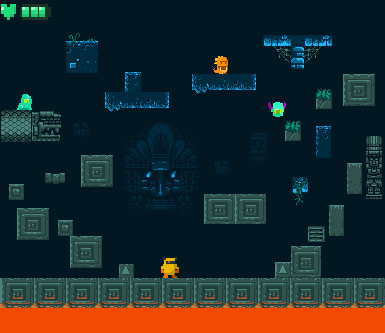
\includegraphics[width=\textwidth, height=15cm]{/home/danhu849/Pictures/game_example.png}}
  \caption{LOFI-exempel för en av spelets nivåer.\label{fig}}
\end{figure}

\section{Kravformulering}
\subsection{Kravuppfyllelse}
Kraven nedan i \emph{kursivt} är minimikrav som spelet minst måste uppfylla för att godkännas. Nedan specificeras också vilka av våra krav som uppfyller minimikraven.

\subsubsection{\emph{ Spelet ska simulera en 2D-värld i realtid. (Måste vara 2-dimensioner)}}
Uppfylls av ska-krav: 1, 3

\subsubsection{\emph{ Minst 3 typer av objekt. Ska finnas flera instanser av minst två av dessa. Till exempel ett spelarobjekt och många instanser av två olika fiendeobjekt.}}
Uppfylls av ska-krav: 3, 5, 11

\subsubsection{\emph{ Ett beteende som måste finnas med är att figurerna (Objekten) ska röra sig över skärmen. Rörelsen kan följa mönster och/eller vara slumpmässig. Minst ett objekt utöver spelaren ska ha någon typ av rörelse.}}
Uppfylls av ska-krav:5, 11

\subsubsection{\emph{ Ska vara enkelt att modifiera banor i spelet. Det ska vara enkelt att lägga till eller ändra banor i spelet. Detta kan exempelvis lösas genom att läsa in banor från en fil (lite som i Sokoban-labben i TDP002), eller genom att ha funktioner i programkoden som bygger upp en datastruktur som definierar en bana. }}
Uppfylls av ska-krav: 12

\subsubsection{\emph{ Spelet ska upplevas som sammanhängande spel som går att spela.}}
Uppfylls av ska-krav: Alla

\subsubsection{\emph{ En figur ska styras av spelaren, antingen med tangentbordet eller med musen. Du kan även göra ett spel där man spelar två stycken genom att dela på tangentbordet (varje spelare använder olika tangenter). Då styr man var sin figur.}}
Uppfylls av ska-krav: 3

\subsubsection{\emph{ Världen (spelplanen) kan antas vara lika stor som fönstret (du kan göra en större spelplan med scrollning, men det blir lite krångligare).}}
Uppfylls av ska-krav: 1, 4

\subsubsection{\emph{ Det ska finnas kollisionshantering, det vill säga, det ska hända olika saker när objekten möter varandra, de ska påverka varandra på något sätt. T.ex kan ett av objekten tas bort, eller så kan objekten förvandlas på något sätt, eller så kan ett nytt objekt skapas.}}
Uppfylls av ska-krav: 3, 8, 9



\subsection{Ska-krav på projektet}
\begin{enumerate}
\item Spelet ska vara en tvådimensionell platformsscroller.
\item Spelet ska ha en startmeny.
\item Spelaren ska kunna röra en spelarfigur sig i alla vädersträck med piltangenterna och kunna stå och hoppa på plattformar.
\item Spelet ska inkludera scrollande nivåer i y-led.
\item Spelaren ska bli jagad av stigande lava.
\item Nivån ska avslutas när man kommer till toppen.
\item När spelaren dör ska en Game Over skärm visas i spelfönstret.
\item Gravitation ska finnas som drar spelaren mot botten av spelskärmen.
\item Spelaren ska kunna avfyra projektiler som försvinner vid kollision med fiender, väggar eller åker utanför banan.
\item Hårdvarukrav: Spelet ska kunna spelas på skolans datorer.
\item Det ska finnas tre olika typer av fiendeobjekt som har olika utseende. En långsam typ, en flygande typ och en hoppande typ.
\item Nivåer ska kunna läsas in från fil.
\end{enumerate}


\subsection{Bör-krav på projektet}
\begin{enumerate}
\item Multiplayer Två spelare kan spela spelet samtidigt.
\item - spelare kan vid multiplayer välja om "friendly fire" ska vara på eller av i spelets inställningar. 
\item Power-ups plockas upp av spelaren genom att spelaren med sin karaktär går in i samma område som power-up ikonen upptar på spelskärmen. Det finns power-ups som ger spelaren tillbaka liv, möjligheten att hoppa högre samt en power-up som gör att spelaren kan hoppa högre.
\item Bakgrunder skiftar i utseende efterhand att spelaren tar sig till högre höjd.
\item Det kan finnas en Level editor som ger spelaren möjlighet att skapa banor.
\item Spelet kan spelas med handkontroll.
\item Animerade sprites (Explosionssprites, rörelse)
\item Fiender kan avfyra av projektiler.
\item Bosstrid, Vid toppen av berget, under striden med bossen slutar lavan att förflytta sig uppåt och stannar kvar vid spelarfönstrets botten.
\item Spelaren kan få highscore på varje nivå.
\item Ljudeffekter kan spelas upp när spelaren tar skada, avfyrar projektiler och dör. Ljud spelas upp när fiender dör.
\item Det finns bakgrundsmusik och musik som spelas i nivåerna.
%\item \subsubsection{Fiendeprojektiler som träffar spelarens projektiler.}
%\subsubsection{Fiendeprojektiler som träffar andra fiendeprojektiler.}
%\subsubsection{Fiendeprojektiler som träffar spelarens projektiler.} 
\end{enumerate}

\subsection{Krav på koden}
\begin{enumerate}
\item    Koden ska följa en accepterad kodstandard. Koden ska gå att kompilera och köra i Ubuntu.
\item    Koden ska vara väldokumenterad. Doxygen ska användas.
\item    "Information hiding" ska användas (ingen åtkomst av instansvariabler utanför klassen).
\item    Designen ska vara modulär med så få beroenden mellan klasser som möjligt.
\item    Det ska finnas en gemensam basklass (Sprite) för alla figurer i programmet. Övriga sprite-figurer ska ärva från denna klass.
\item    Det ska finnas abstrakta metoder, åtminstone för er Sprite-hierarki.
\item    Main-funktionen ska vara liten, huvuddelen av spelet ska finnas i de klasser ni designar. Ett exempel på en lämplig main-funktion:

    int main {
       Game game;
       game.run();
       return 0;
    }
        

\item    Grafiken ska realiseras med hjälp av SFML.
\item    Tillsammans med koden ska en Makefile lämnas in. Handledaren ska kunna köra koden i terminalen med hjälp av denna Makefile.
\end{enumerate}



\end{document}

%%% Local Variables:
%%% mode: latex
%%% TeX-master: t
%%% End:
